\documentclass[letterpaper,12pt,oneside]{book}


\usepackage[utf8]{inputenc}

\usepackage[spanish,es-nodecimaldot,es-tabla]{babel}

\usepackage{graphicx}

\usepackage{natbib}  % Usando paquete para citas

\usepackage{amsmath} % Notación

\usepackage{amssymb}

\usepackage{amsthm}  % Definiciones

\usepackage{longtable}

\usepackage{todonotes}   % insert [disable] to disable all notes


\newcommand{\note}[4][]{\todo[author=#2,color=#3,size=\scriptsize,fancyline,caption={},#1]{#4}} % default

\newcommand{\ximena}[2][]{\note[#1]{Ximena}{green!40}{#2}}

\newcommand{\vic}[2][]{\note[#1]{Vic}{orange!40}{#2}}

\newcommand{\diego}[2][]{\note[#1]{Diego}{blue!40}{#2}}

\newcommand{\Ximena}[2][]{\ximena[inline,#1]{#2}\noindent}

\newcommand{\Vic}[2][]{\vic[inline,#1]{#2}\noindent}

\newcommand{\Diego}[2][]{\diego[inline,#1]{#2}\noindent}



\graphicspath{{./img/}}


\newtheorem{definition}{Definición}


\begin{document}

	\bibliographystyle{acl_natbib}  % Cargando estilo de bibliografia

	
	\author{Diego Alberto Barriga Martínez}

	\title{Etiquetador automático de la morfología del otomí usando predicción estructurada}

	\tableofcontents

	\maketitle

	
	% TODO: Pasar todo lo del protocolo aquí

	% Utilzar el tiempo pasado 

	
	\chapter{Introducción}

	
	% Capitulo corto con el objetivo, hipótesis y tocar los temas del marco teorico de forma muy superficial. Se definen en el marco teorico

	
	\section{Problemática}

	
	% TODO: Cambiar las citas a bibtex

	El NLP es un área de la computación que permite reconocer, procesar e interpretar el lenguaje humano dentro de un sistema computacional. El objetivo de esta área es hacer que las computadoras realicen tareas que involucran el lenguaje humano. Algunas tareas generales consisten en permitir la comunicación humano-máquina, o simplemente hacer un exitoso procesamiento de texto o voz humanos. (Jurafsky \& Martin, 2014). Ejemplos de aplicación actuales son los traductores automáticos, asistentes personales que reconocen voz, motores de búsquedas en Internet, análisis de sentimientos en textos,  síntesis de voz, etiquetado de textos y muchas más aplicaciones.

	
	% Voy de lo mas general a lo particular

	Una de las tareas más populares de NLP es el etiquetado automático de textos. Este etiquetado puede realizarse a diferentes niveles lingüísticos, por ejemplo, morfosintáctico (Part-Of-Speech tagging), sintáctico (parsing), morfológico, etc.  El nivel morfológico tiene que ver con la estructura interna de las palabras (Haspelmath y Sims, 2013); en particular, existe un tipo de etiquetado, de gran importancia para el análisis lingüístico, llamado glosado que asigna etiquetas a las unidades que conforman a una palabra. 

	
	% Hablando de ML

	Para lograr lo anterior, los enfoques actuales aplican técnicas de ML. El ML es un subcampo de la Inteligencia Artificial (IA), que constituye un enfoque de resolución de problemas caracterizado por estimar una solución a partir de la experiencia (Mitchell, 1997).  La experiencia se refiere a datos etiquetados (ejemplos) que permiten inferir un modelo estadístico de aprendizaje. Entre los métodos de ML ampliamente utilizados se pueden mencionar las Support Vector Machines (SVMs), árboles de decisión, o bien los modelos gráficos, como las redes neuronales o los métodos generativos, solo por mencionar algunos. Para las tareas de etiquetado en NLP generalmente se utilizan modelos gráficos supervisados, por ejemplo, modelos ocultos de Markov (Hidden Markov Models, HMM).

	
	% Introduccion de la problematica

	No obstante, el lenguaje natural es complejo y dinámico, ya que tiene fenómenos que hacen que las tareas de reconocimiento, generación y procesamiento se vuelvan difíciles para las computadoras. Adicionalmente, existen escenarios donde estos métodos no son efectivos como es el caso de las lenguas de bajos recursos, que son lenguas que tienen pocos recursos digitales con los que trabajar. Por ejemplo, si se tienen pocos datos iniciales para el entrenamiento del modelo de aprendizaje las predicciones serán poco precisas o equivocadas. Los bajos recursos son un escenario común en México donde, a pesar de que existe una rica diversidad lingüística, gran parte de las lenguas originarias no poseen contenido web ni publicaciones digitales y por tanto carecen también de tecnologías del lenguaje.  El escenario mencionado anteriormente supone un reto para los métodos de aprendizaje convencionales, que requieren de grandes cantidades de datos de entrenamiento para funcionar correctamente. Por lo tanto, es un importante reto de investigación desarrollar aproximaciones que funcionen con lenguas de escasos recursos. En particular, nos enfocaremos en el glosado automático del  otomí, una lengua con gran riqueza morfológica y con escasez de recursos digitales.

	
	El glosado puede ser un primer paso para el desarrollo de más tecnologías del lenguaje; no solo para el otomí, que presenta un grado de extinción acelerada (CDI), sino para las 68 agrupaciones lingüísticas que se hablan en México.

	
	\subsection{Lengua otomí}

	
	En esta sección se menciona los lugares donde se describe el idioma otomí de forma somera, se mencionan algunos lugares donde es hablado el otomí y características fundamentales de la lengua.

	
	\subsection{Origen}

	
	% Pie de pagina, no meter cosas tangenicales. Citar esta definicion

	La palabra otomí es de origen náhuatl (singular: \textit{otomitl}, plural: \textit{otomí}). Por otra parte, los otomíes se nombran a sí mismos \textit{ñähñu}\footnote{Existen organizaciones indígenas, como el Consejo de la Nacionalidad Otomí, que escriben la auto-denominación como hñätho hñähñu y también ñätho ñähño. Sin embargo, esta auto denominación puede variar.}, que significa "los que hablan otomí".

	
	Los grupos indígenas que hablan el idioma otomí se encuentran en diversas partes del territorio mexicano como: Estado de México, Querétaro, Hidalgo, Puebla y Veracruz \citep{barrientos2004otomies}. El otomí es una lengua indígena una gran variación dialectal que depende de su distribución geográfica.

	
	En el Estado de México el pueblo \textit{ñähñu} está disperso por varios municipios tales como: Toluca, Lerma, Chapa de Mota, Aculco, Amanalco, Atizapán de Zaragoza, por mencionar algunos. En otros municipios como Naucalpan, Ecatepec, Nezahualcóyotl y Tlalnepantla se pueden encontrar hablantes por efectos de la migración. Según \citet{barrientos2004otomies} la población total de hablantes otomíes en el Estado de México supera los cien mil, sin embargo, datos actuales .

	
	En concreto existen \textbf{nueve} variantes del otomí y cabe recalcar que dicha variación puede presentarse incluso dentro del mismo estado. Tan solo el Estado de México presenta tres variantes del otomí: El otomí de Tilapa, hablado en el municipio de Santiago Tianguistenco; el Otomí de Acazulco, del municipio de San Jerónimo Acazulco; y el Otomí de Toluca, de San Andrés Cuexcontitlán.

	
	\section{Objetivo}

	
	Diseñar e implementar un etiquetador morfológico para el otomí basado en técnicas de

	Procesamiento del Lenguaje Natural (Natural Language Processing, NLP) con Aprendizaje de Máquina (Machine Learning, ML). En particular, se hará énfasis en métodos de aprendizaje estructurado débilmente supervisados. Específicamente, se aplicará \textit{Conditional Random Fields (CRF)} para etiquetado morfológico (glosado) del otomí, una lengua de bajos recursos.

	
	\section{Hipótesis}

	
	Se espera obtener un modelo que produzca glosa para el otomí, generada automáticamente, con base en el entrenamiento con pocos ejemplos previamente etiquetados. Al obtener una buena exactitud en la predicción automática de glosa se apoyaría a los anotadores humanos a reducir trabajo repetitivo y exhaustivo. Además, se espera obtener avances de una metodología adaptable a un mayor número de lenguas mexicanas. Sería deseable que esta metodología experimental pueda ser replícale en otras lenguas habladas en México.

	
	\chapter{Avances en etiquetadores automáticos}

	
	% Mencionar los bajos recursos

	
	\section{Marco teórico}

	
	% Se tiene que explicar los conceptos de low resouces 

	% -NLP

	% -Machine learning

	% .Etiquetadores a diferentes niveles lingüísticos

	% -Etiquetadores a nivel morfológico

	% -modelos gráficos

	% Que es un etiquetador 

	% Que es la morfología 

	% que es la glosa

	% Low resources

	% Algoritmo L-BFGS

	% L1 - L2

	
	\subsection{NLP}

	% Introduccion

	
	\subsection{Etiquetadores}

	
	\subsection{ML}

	
	\subsection{Modelos gráficos}

	
	% Los límites de los modelos gráficos para bajos recursos

	
	% Cierre de los modelos graficos y comenzar a hablar de CRF

	% No perder de vista que los CRFs son modelos graficos pero con ventajas

	
	\subsubsection{Los límites de los modelos gráficos en para bajos recursos}

	
	En este capítulo se explicará qué ventajas tienen los \emph{Conditional Random Fields (CRF)} sobre otros modelos de aprendizaje, se mencionan formalmente los elementos fundamentales que describen los \emph{CRF's}.

	
	En lingüística computacional una tarea de interés es el procesamiento estadístico del lenguaje natural, en particular, el etiquetado y segmentación de secuencias de datos. En ese sentido, es habitual la utilización de \textbf{modelos generativos}, cómo los \textit{Hidden Markov Models (HMMs)}, o \textbf{modelos condicionales}, como los \textit{Maximum Entropy Markov Models (MEMMs)}.

	
	Por una parte, los modelos generativos intentan modelar una probabilidad conjunta $P(x,y)$ sobre observaciones y etiquetas. Para definir esta probabilidad conjunta se necesita enumerar todas las observaciones posibles. Las limitantes de este enfoque son de diversas índoles como las grandes dimensionalidades en el vector de entrada $X$, la dificultad de representar múltiples características que interactúan unas con otras y dependencias complejas que hacen la construcción de la distribución de probabilidad un problema intratable con un enfoque computacional.

	
	Por otro lado, una solución a las limitantes de los modelos generativos es un modelo condicional. Estos modelos no son tan estrictos como los primeros al momento de asumir independencias en las observaciones. Los modelos condicionales especifican la probabilidad de posibles etiquetas dada una secuencia de observación.

	
	Consecuencia de lo anterior, no se gasta esfuerzo en modelar las observaciones, dado que en al momento de realizar pruebas estas observaciones son fijas. Segundo, la probabilidad condicional puede depender de características arbitrarias y no dependientes de la secuencia de observación sin forzar al modelo a tomar en cuenta la distribución de estas características, permitiendo que el modelo sea tratable \citep{lafferty2001conditional}.

	
	Un ejemplo de estas ventajas con los \textit{MEMMs} que son modelos secuenciales de probabilidad condicional. Sin embargo, estos modelos y otros que son no generativos, de estados finitos y que son clasificadores basados en el estado siguiente comparten una debilidad llamada \emph{label bias problem}. \citet{lafferty2001conditional} define que existe el \emph{label bias problem} cuando "las transiciones que dejan un estado compiten solo entre sí, en lugar de entre todas las demás transiciones en el modelo".

	
	Dado que las transiciones son las probabilidades condicionales de los siguientes posibles estados una observación puede afectar cuál será el estado siguiente sin tomar en cuenta que tan adecuado será este. Por tanto, se tendrá un sesgo en los estados con menos transiciones de salida.

	
	\subsection{Conditional Random Fields}

	
	Como menciona \citet{sutton2012introduction} modelar las dependencias entre las entrada puede conducir a modelos intratables, pero ignorar estas dependencias puede reducir el rendimiento.

	
	Dado el que problema abordado en este trabajo, dónde se requiere del etiquetado de secuencias y es en contexto de bajos recursos lingüísticos, se hace necesario utilizar un enfoque más conveniente.

	
	Los \textit{Conditional Random Fields (CRFs)} son un framework para la creación de modelos probabilístico utilizado en técnicas de aprendizaje estructurado. Tienen las ventajas de los \textit{MEMMs} y, en principio, solucionan el \emph{label bias problem}. El framework tiene un solo modelo exponencial para la probabilidad conjunta de todas las secuencias de las etiquetas de salida dada la secuencia de observación. En contraste los \emph{MEMMs} usan modelos exponenciales para cada probabilidad condicional de los estados siguientes dado el estado actual.

	
	Formalmente \citet{lafferty2001conditional} definen los \textit{CRFs} como a continuacion se enuncia:

	
	\begin{definition}

		Sea $G = (V,E)$ una gráfica tal que $\mathbf{Y} = (\mathbf{Y}_{v})_{v \in V}$, entonces esa $\mathbf{Y}$ es indexada por los vertices de $G$. Entonces $(\mathbf{X}, \mathbf{Y})$ es un \textsf{conditional random field} en caso de que las variables aleatorias $\mathbf{Y}$ se condicionen por $\mathbf{X}$, la variable aleatoria $\mathbf{Y}_{v}$ cumple la \textit{propiedad de Markov} con respecto a la gráfica: $p(\mathbf{Y}_{v}|\mathbf{X},\mathbf{Y}_{w},w \ne v) = p(\mathbf{Y}_{v}|\mathbf{X},\mathbf{Y}_{w},w \sim v)$, dónde $w \sim v$ significa que $w$ y $v$ son vecinos en $G$.

	\end{definition}

	
	En esta tesis, para el modelado de secuencias, se utiliza la forma más sencilla de la gráfica $G$ dónde es una cadena simple o línea. Esto quiere decir que $G = (V = \{1,2,...m\}, E = \{(i,i+1)\})$. A este tipo de \textit{CRFs} se les conoce como \textit{linear-chain CRFs}. Como menciona \citet{lafferty2001conditional} "si la gráfica $G = (V,E)$ de $\mathbf{Y}$ es un árbol (del cual una cadena es el ejemplo más sencillo), los cliques??? son los límites y vertices. Entonces, por el teorema de los \textit{random fields} \citep{hammersley1971markov}, la distribución conjunta sobre las etiquetas de secuencias $\mathbf{Y}$ y $\mathbf{X}$ tiene la forma:

	
	
	% TODO: Poner tag

	% TODO: Explicar esta ecuacion sobre que es son las lambdas, porqeu hay dos sumandos, porque el simbolo de proporcionalidad, 

	\begin{equation}

	p{_{\theta}}(y|x) \propto \exp \bigg( \sum\limits_{e \in \mathbf{E},k} \lambda_{k}f_{k}(e,\mathbf{y}|_{e},\mathbf{x}) + \sum\limits_{v \in \mathbf{V},k}\mu_{k}g_{k}(v,\mathbf{y}|_{v},\mathbf{x}) \bigg)

	\end{equation}

	
	% TODO: Mencionar la ecucacion

	% TODO: Descripcion de la estimacion de parametros y caracteristica de la funcion de perdida

	
	De la ecuación  se destacan $f_{k}$ y $g_{k}$ que representan las \textit{feature functions}. Estas están definidas y son fijas. Las \textit{feature functions} de está tesis serán descritas más adelante. 

	
	\section{Estado del arte}

	
	Los \textit{CRFs} han sido utilizados para la clasificación de regiones en una imagen, estimar el puntaje en un juego de Go, segmentar genes en una hebra de ADN y análisis sintáctico de lenguaje natural en un texto por mencionar algunas \citep{sutton2012introduction}.

	
	% Papers que hablen del tema de etiquetado automatico 2010 para acá

	
	% Redes neuronales,

	% Mencion de trabajo y papers actuales hacen algo similar

	% Lezgi

	
	
	\chapter{Etiquetador morfológico para el otomí (Metodología)}

	
	En este capitulo se describe el corpus utilizado en este trabajo, se mostrará la arquitectura propuesta para la generación automática de glosa para el idioma otomi. Adicionalmente, se explicará el diseño e implementación del \textit{pipeline} que incluye, entre otras cosas, la determinación de las \textit{feature functions}.

	
	%TODO: Descripcion de la estimacion de parametros y caracteristica de la funcion de perdida

	
	Los CRFs muestran claras ventajas sobre otros métodos de aprendizaje basados en gráficas. Su habilidad de tomar las virtudes de los modelos generativos y de los modelos condicionales presentan a este \textit{framework} como una opción para el contexto de \textit{low resouces} que nos impone, como se describirá más adelante, el tamaño del corpus.

	
	
	% Particularidades del corpus (Analisis cualitativo y cuantitativo)

	\section{Corpus: otomí de Toluca}

	
	% Siempre ir de lo general a lo particular

	
	% Tipo de otomi y caracteristicas de la variante

	La clasificación lingüística introduce al otomí dentro de las lenguas otomianas, las cuales a su vez pertenecen a la rama otopame de la familia otomangue \citep{barrientos2004otomies}. Cada variante muestra particularidades fonológicas, morfológicas, sintácticas y léxicas. En el tratamiento de textos por medio de técnicas de \textit{NLP} se requiere que estos estén normalizados y homogéneos. Lo anterior propicia la obtención del mejor desempeño posible en los diversos métodos de aprendizaje automático.

	
	% Otomi en general, Familia y rama

	En este trabajo se utilizó un corpus en otomí que, además, cumple la característica de estar glosado. Se trabaja con la variante del otomí de Toluca de la región de San Andrés Cuexcontitlan.

	
	% De donde vienen los textos, quien lo glosa y quien lo recolecta

	Esta tesis recogío un corpus basado en el trabajo de \citet{lastra1992otomi} titulado \emph{El otomí de Toluca} y que a su vez fue  etiquetado y glosado manualmente por el lingüista Víctor Germán Mijangos de la Cruz\footnote{TODO: Liga del repo}. Este corpus es un subconjunto del corpus paralelo español-otomi que se encuentra en la plataforma web Tsunkua\footnote{https://tsunkua.elotl.mx/} TODO: ¿Como se cita?. El subconjunto del corpus utilizado en la sección experimental está descrito en la tabla \ref{table_corpus_length:1} y en la tabla \ref{table_corpus_text:1}. 

	
	% Describir las tablas en el texto

	% Tokens y tipos de Palabras

	
	% Numero de etiquetas diferentes

	\begin{table}

		\centering

		\begin{tabular}{c | c}

			\textbf{Categoría} & \textbf{Cuenta} \\ \hline

			Tokens (POS) & 8578\\

			Tipos (POS) & 44\\

			Tokens (Glosa) & 14477\\

			Tipos (Glosa) & 112\\

			Oraciones etiquetadas & 1786 \\ 

		\end{tabular}

		\caption{Tamaño del corpus}

		\label{table_corpus_length:1}

	\end{table}

	
	\begin{table}

		\centering

		\begin{tabular}{ c | c }

			\textbf{Textos} & \textbf{Número} \\ \hline

			Narrativos & 32 \\

			Dialogados & 4  \\

			\textbf{Total de textos}  & 36 \\

		\end{tabular}

		\caption{Textos del corpus}

		\label{table_corpus_text:1}

	\end{table}

	
	Los textos que componen el corpus fueron construidos a partir de las aportaciones de diez hablantes distintos de entre diez y setenta y tres años, de los cuales, siete son de sexo femenino y tres masculino \citep{lastra1992otomi}. 

	
	% TODO: Caracteristicas escenciales que tiene que ver con el etiquetado POS de las lenguas otomies

	% TODO: Descripcion detalla del etiquetado POS

	
	% Descripcion del corpus (tipos, tokens)

	% Tokens y tipos de Palabras

	
	% Reorganizar esto

	% Seccion sin seccion de POS, glosa, Bio labels sin tablas

	% tipos, tokens, distribucion 

	% Citar el estandar de etiquetas https://www.eva.mpg.de/lingua/pdf/Glossing-Rules.pdf

	
	% Mencionar que hay etiquetas en si mismas pero quitarlas de la tabla

	
	\begin{table}

		\centering

		\begin{tabular}{| c | c | c | c | c |}

			\hline

			v & obl & det & cnj & dem \\ 

			unkwn & n & neg & p.loc & prt \\

			conj.adv & dim & gen & cond & it \\

			lim & aff & loc & pascuala & toluca \\

			chente & dec & conj & chalma & mexico \\

			tapanco & cord & san & cnj.adv & regular/v \\

			adv & juan & andrés & buena.vista & nada.más \\

			zapata & calvario & bautisterio & adj & cristo \\

			emilio & pato & luis & mextepec & \\

			\hline

		\end{tabular}

		\caption{POS} 

		\label{table_pos_types}

	\end{table}

	
	
	% Mencionar que hay etiquetas en si mismas pero quitarlas de la tabla

	
	\begin{table}

		\centering

		\begin{tabular}{| c | c | c | c | c | c | c |}

			\hline

			stem & det & 3.cpl & psd & lim & prag & 3.icp \\

			det.pl & 1.icp & 3.pot & ctrf & 1.pot & pl.exc & 1.cpl \\

			dem & 1.pss & dim & pl & 1.obj & ila & 2.icp \\

			1.prf & 3.cnt & 3.obj & loc & mod & 1.cnt & 3.pls \\

			muy & prt & it & dual.exc & 3.prf & 3.icp.irr & 3.pss \\

			2.pss & 1.enf & med & dual & p.loc & 2.cnt & 2 \\

			3.imp & int & neg & 1.icp.irr & 1.cpl.irr & 2.obj & pues \\

			que & aum & 1.pls & y & 2.cpl & toluca & 2.prf \\

			aqui & gen & hasta & com & 2.pot & adj & cuando \\

			cond & como & 3.cpl.irr & 1.sg & encl & por.que & solo \\

			agujerear/v & mientras & 3.sg & uno & 3.pss.pl & spt & mexico \\

			1.irr & mucho & 2.enf & conj.adv & pueblo & animal.de.dios & caus \\

			tiempo & con & lugar/v & chico & eh & para & comp \\

			prf & dónde & dist & mov & pascuala & 3.irr & loco \\

			coraje & si & det.dem & dcl & nom & chente & vez \\

			rapido & maria & 2.icp.irr & tal.vez & mujer/v & dios & lig \\

			\hline

		\end{tabular}

		\caption{Glosa} \vic{Explicar qué significa cada etiqueta}

		\label{table_gloss_types}

	\end{table}

	
	\subsection{Tokens}

	
	\begin{table}

		\centering

		\begin{tabular}{c | c}

			\textbf{Etiqueta} & \textbf{Tokens} \\ \hline \hline

			v & 2596 \\

			obl & 2447 \\

			det & 975 \\

			cnj & 837 \\

			dem & 543 \\

			unkwn & 419 \\

			n & 273 \\

			neg & 178 \\

			p.loc & 81 \\

			prt & 49 \\

		\end{tabular}

		\caption{POS (Primeros 10)}

		\label{table_pos_tokens}

	\end{table}

	
	
	\begin{table}

		\centering

		\begin{tabular}{c | c}                            

			\textbf{Etiqueta} & \textbf{Tokens} \\ \hline \hline

			stem & 7527 \\

			det & 733 \\

			3.cpl & 450 \\

			psd & 418 \\

			lim & 374 \\

			prag & 362 \\

			3.icp & 346 \\

			lig & 289 \\

			det.pl & 271 \\

			1.icp & 270 \\

		\end{tabular}

		\caption{Glosa (Primeros 10)}

		\label{table_gloss_tokens}

	\end{table}

	
	
	% Grafica de Zipf para las etiquetas POS

	% Distribucion de etiquetas

	\subsection{Distribución de etiquetas}

	
	\begin{figure}

		\centering

		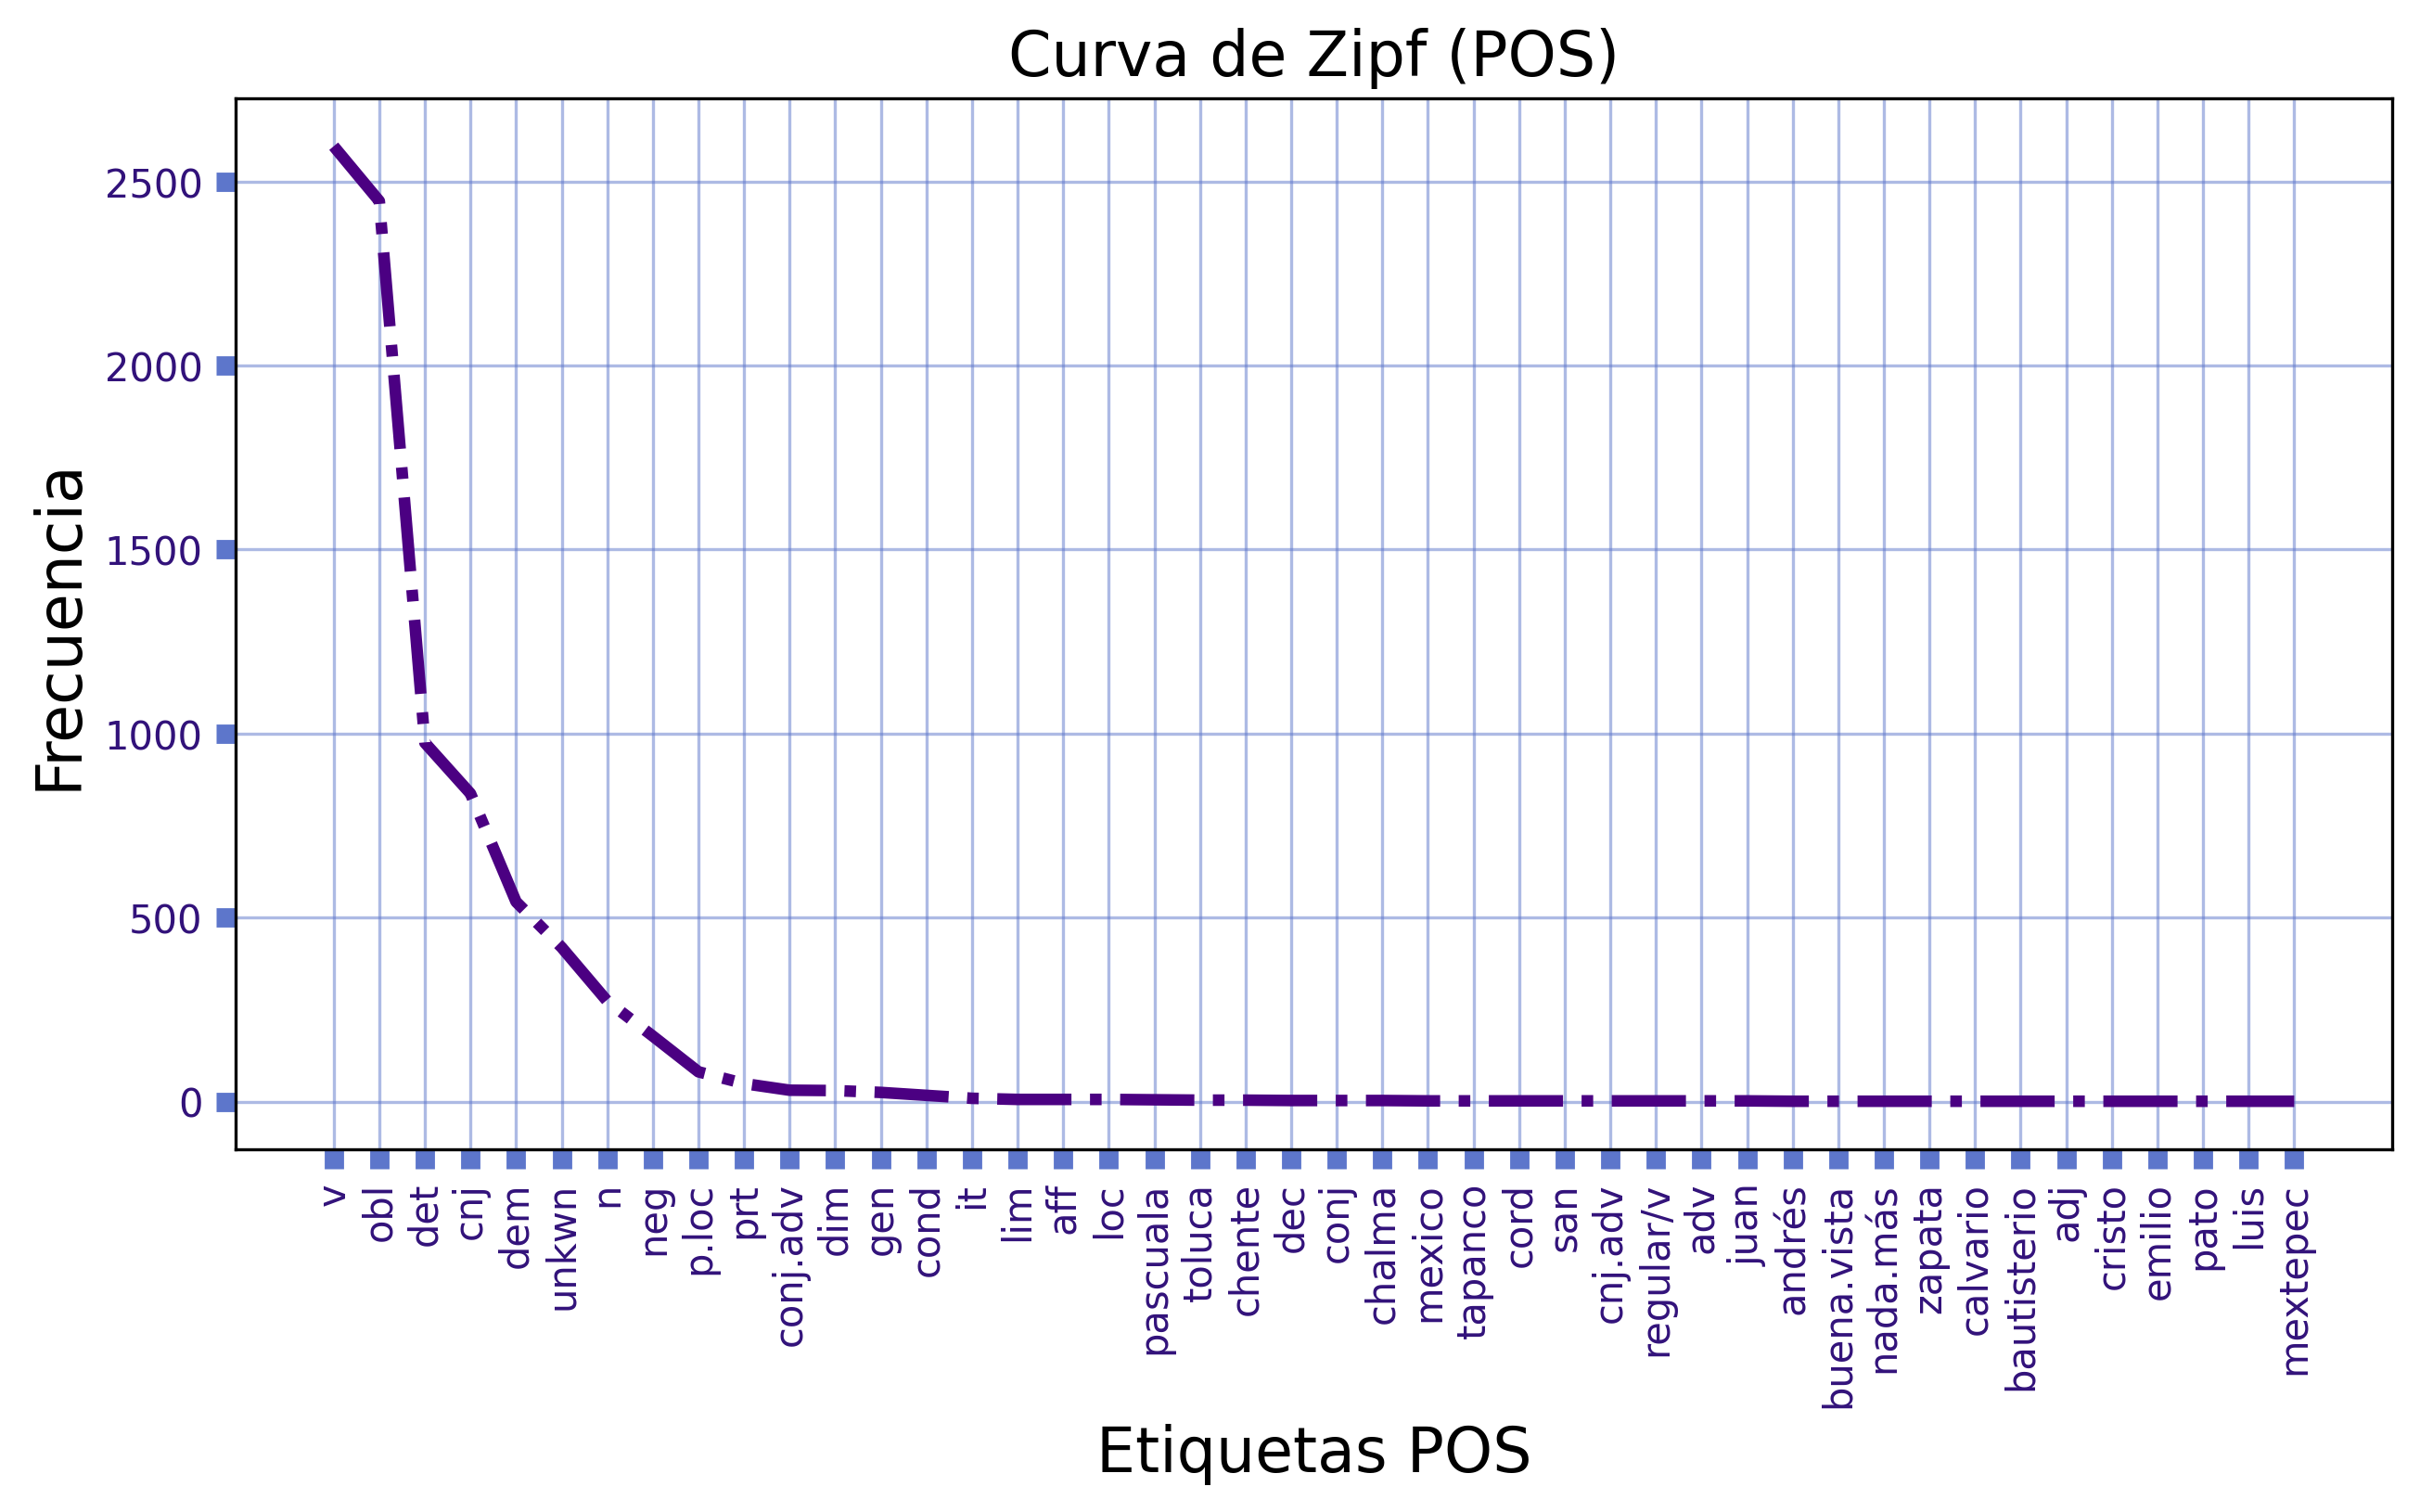
\includegraphics[width=\textwidth]{zipf_pos}

		\caption{Distribución de etiquetas POS}

	\end{figure}

	
	\begin{figure}

		\centering

		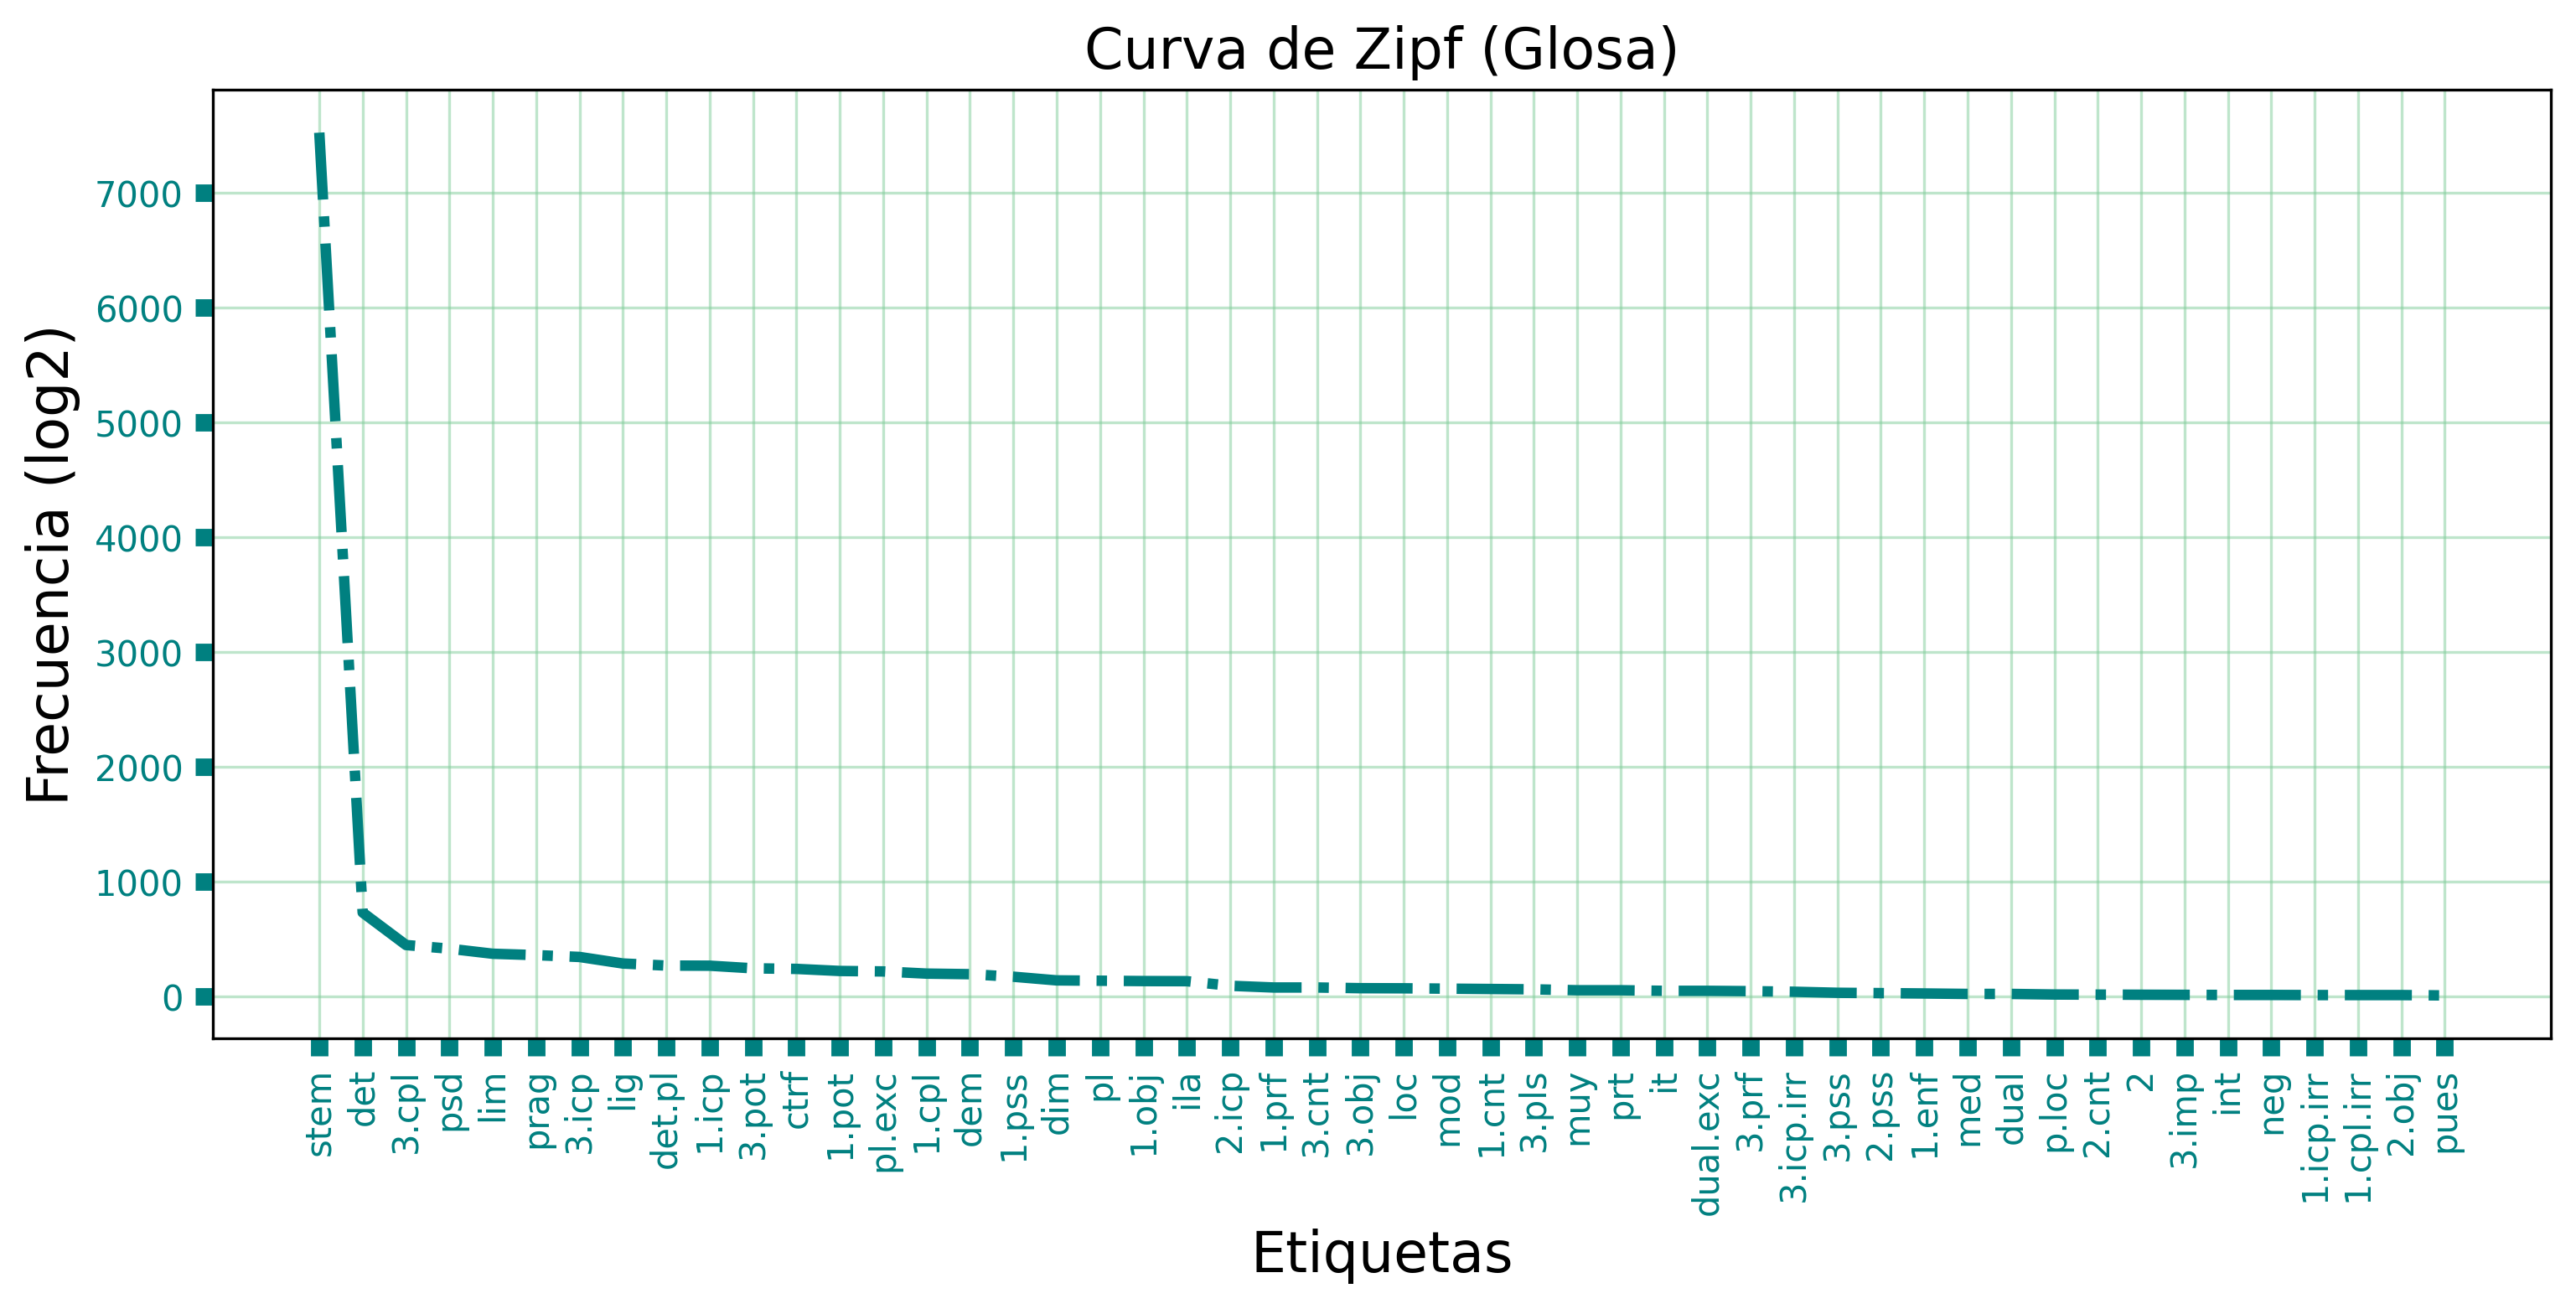
\includegraphics[width=\textwidth]{zipf_gloss}

		\caption{Distribución de glosa (primeras 50)}

	\end{figure}

	
	%5. Tipos de POS y cuantos de cada uno

	
	%Descripción general del corpus. Orientar que la arquitectura esta enfocada en

	%resolver el problema de low resources

	
	\section{Arquitectura}

	
	% Definir el metodo en funcion del marco teorico

	% Diagrama de la arquitectura

	% ¿Que es X y Y?

	% Feature functions

	% Como se decidieron

	% ¿Porque estas caracteristicas son reelevantes?

	% Que es para nosotrxs una FF

	% Experimentos quitando features functions

	% Diagram de donde se encuentran estos elementos en la arquitectura

	% Como se calculan lambdas y mu

	% Variacion de hiperparametros

	% Descripcion de que variaciones se hicieron

	% Hablar de L1 y L2 con ciertas combinaciones

	% Mostrar el base line y compararlo

	% Metodo de regularizacion y optimización

	% Mencionar que se usará un base line

	% ¿Cómo se hizo lo que se hizo?

	% Preprocesamiento del corpus

	% 

	
	Para esta tesis proponemos una arquitectura de aprendizaje

	estructurado  supervisado utilizando un método gráfico, Conditional

	Random Field (CRF), que permitirá la predicción de secuencias que describen

	las unidades morfológicas (glosa) dentro de una palabra en otomí

	
	Se utilizaron CRFs para predecir secuencias de glosa, que será la salida $Y$

	dadas las observaciones $X$ que son el texto previamente glosado. Puntualmente,

	se utiliza el modelo gráfico 1st-order Markov CRF with dyad features.

	Adicionalmente, es utilizado el algoritmo de aprendizaje de Limited-memory

	Broyden-Fletcher-Goldfarb-Shanno (L-BFGS) como se menciono en TODO.

	
	% TODO: Debe tener un lugar en el estado del arte

	\ximena{Tener bien claro cuál es nuestra hipótesis, separarnos un poco del trabajo de lezgi}

	Con base en el trabajo previo para del idioma Lezgi \citep{moeller2018automatic} se plantea como hipótesis que dado el tamaño del corpus y la glosa que contiene

	se obtendrá texto correctamente glosado con una precisión de al menos 80\%. El objetivo de esta arquitectura con CRF realizar un etiquetador automatico  que bajo ciertas condiciones etiquete glosa automaticamente. 

	Ya que el resultado esperado es la generación de etiquetas que, en principio,

	dependen unas de otras un método basado en grafos como los CRF puede ser

	adecuado. Se definieron de aprender un conjunto de feature functions que

	describen TODO el contexto y brindan información útil para la fase de

	entrenamiento.

	
	El modelo de aprendizaje semi-supervisado, para la generación de glosa para

	el otomí se describe a continuación:

	
	% TODO: HACER ESTA PARTE POR PUNTOS MAS BREVES Y CADA PUNTO HACERLO SECCION Y PROFUNDIZAR

	
	\begin{itemize}

		\item Obtener el corpus en otomí previamente glosado y obtenerlo en un

		formato que especifique la información de las oraciones a nivel

		de letra especificando su Bio Label.

		\item Los CRF toman como entrada los datos $X$ que corresponden al

		corpus en otomí introducido en las feature functions asociados

		de forma biyectiva con la etiqueta Bio Label que le corresponde.

		Con base en esto se entrenará un modelo que busque maximizar el

		logaritmo de verosimilitud con el método de aprendizaje L-BFGS

		\item Posterior se obtendrá un modelo entrenado con el que se generarán

		etiquetas de glosa para el otomí. Por lo tanto, el modelo

		recibirá párrafos de texto en otomí y retornará el texto

		glosado.

		\item Se considera exitosa la predicción si se logra maximizar la

		correcta clasificación de las secuencias de salida. Para

		determinar si la predicción fue exitosa se utilizaron técnicas

		típicas de ML como K-folds que consiste en tomar K fragmentos

		de los datos de entrada para utilizarlos para probar el modelo

		y así obtener una precisión, recall y F-score.

	\end{itemize}

	
	
	% TODO: Resumen al final (pasos de todo lo que se hizo)

	
	\subsection{Feature functions}

	
	\subsection{Hardware utilizado}

	
	En la fase de experimentación fue utilizado el paquete \textsf{python-crfsuite} que es un \textit{binding} de la implementación de \citet{CRFsuite} para CRFs para lenguaje de programación \textit{Python} en su versión \textit{3.7}. La fase de experimentación corrió en una maquina con un procesador \textsf{Intel i7-7700HQ @ 3.800GHz} con \textsf{16 GB} de memoria principal. En promedio una corrida de entrenamiento y evaluación \textit{K-folds} con \textit{k=10} tomó 52 minutos.

	
	\chapter{Experimentación y Resultados}

	
	
	% Mostrar la comparación a profundidad del baseline con todos los experimentos

	% Demostrar que lo que propusimos fue mejor

	% Cualitativos y cuantitativos

	% Hablar del Baseline y como mejoró con mas features

	% Definir como plantear la historia: 

	% De lo mas basico (baseline) y ver como lo mejoramos con las feature functions

	% El conocimiento lingüístico ayuda a mejorar

	
	\section{Corpus de evaluación}

	
	Aquí se habla del K fold y de como se introdujo el corpus retador.

	
	\section{Análisis de resultados}

	
	\chapter{Conclusiones}

	
	\bibliography{tesis}

	
\end{document}